% !TEX root = ../main.tex
\section{State of the Art}

 {\color{red} Add new benchmarks}
\subsection{Code Review Automation}

Automated code review solutions address a diverse range of tasks aimed at
enhancing the quality and efficiency of the code review process. These
solutions take the form of a variety of functions, including analyzing code
changes, classifying modifications, performing quality checks, sentiment
analysis, retrieving similar code fragments, and generating revised code
suggestions.

\subsubsection{Code Change Analysis}

The field of code change analysis focuses on extracting meaningful information
from submitted code modifications to assist reviewers in their assessment
process. Several key techniques have been developed to achieve this goal.

One technique, known as \textit{Decomposing Tangled Commits}, involves
automating the process of dividing large, multi-purpose commits into smaller,
more cohesive changes. This decomposition makes the review process more
manageable by allowing reviewers to focus on individual, well-defined updates
rather than tackling complex, entangled changes. This technique is particularly
useful when large commits obscure the individual purposes of code changes, as
it allows reviewers to understand and assess each part with greater clarity
\cite{barnett:icse2015,tao:msr2015,wang:ase2019}.

Another significant approach is \textit{Predicting Salient-Class}, which seeks
to identify the primary class or component within a commit that has the most
substantial impact on other changes. By isolating this ``salient'' class,
automated tools provide a starting point for reviewers, helping them prioritize
their inspection within a complex set of modifications. This approach enhances
navigation and efficiency, particularly in large codebases where identifying
the most influential elements can be challenging \cite{huang:tse2020}.

Finally, the technique of \textit{Linking Similar Contributions} enhances
review consistency by identifying and connecting similar code changes across
different reviews. This linking process enables automation tools to highlight
potentially duplicated or interrelated code sections, making it easier for
reviewers to ensure coherence and avoid redundant modifications. By surfacing
these relationships, reviewers gain better context on previously reviewed
changes, thus promoting consistency across the codebase \cite{wang:ist2021a}.

\subsubsection{Code Change Classification}

Research in code change classification provides reviewers with valuable
insights by categorizing entire code changes before the review process begins.
This pre-classification helps reviewers focus on changes based on their
likelihood of being merged or on the review effort required. One of the main
tasks in this area involves predicting the probability that a code change will
be approved and eventually merged. Automated tools that assess
\textit{Approval/Merge Likelihood} help reviewers prioritize changes that may
require closer inspection due to potential disagreements or greater impact
\cite{fan:emse2018,islam:ist2022,shi:2019,wu:kbs2022,wu2022contrastive,li:fse2022}.

In addition to merge likelihood, other research has focused on identifying
changes that may require extensive review or can be handled quickly. By
flagging \textit{Large- or Quick-review Code Changes}, these tools help
reviewers manage their time effectively. For example, Wen \etal
\cite{wen:icsme2018} introduced the BLIMP Tracer tool, which uses impact
analysis to identify changes affecting critical parts of the project.
Similarly, Wang \etal \cite{wang:ist2021a} expanded this idea to develop
automated methods for identifying changes that may require a high review
effort, while Zhao \etal \cite{zhao:emse2019} focused on finding changes that
can be reviewed or rejected quickly. Like the merge likelihood predictions,
these classifications assist reviewers in deciding which changes to prioritize
based on the expected review time and importance.

\subsubsection{Revised Code Generation}
\label{sub:revised}
Given a code snippet and its associated review, the goal is to find or generate an
implementation that meets the requirements described in the review, which is
often expressed in natural language.

Tufano \etal \cite{tufano:icse2021} tackled the task from two prospectives: (i)
generating the revised code only given the submitted code, \ie, without any
input from the reviewer; (ii) generating the revised code with the specific
goal of implementing the reviewers suggestion. They demonstrated feasibility of
using deep learning to partially automate code reviews but also limitations,
such as data noise and modest accuracy, paving the way for further research.

The approach leverages a dataset of 17,194 triplets mined from Java open-source
projects on GitHub and Gerrit. This dataset included code review examples with
reviewer comments and revised code. Each triplet had the structure $<m_s,
	c_{nl}, m_r>$, where $m_s$ is a method submitted for review, $c_{nl}$ is a
reviewer’s comment in natural language recommending changes, and $m_r$ is the
revised method that implements $c_{nl}$’s suggestions.
%For the task of code review generation, we are only interested in $m_s$ and $c_{nl}$. 
After some filtering, they applied abstraction to the code (both $m_s$ and
$m_r$), a representative example of this can be found in
Figure~\ref{fig:abstraction}. Although this approach does in fact solve the
vocabulary size issue, it creates a new one: namely the out-of-vocabulary
issue, where the expected revised code might introduce a new variable/method
that the abstraction has never heard of, and therefore cannot invent. As a
result, any instances featuring a revised method that introduces new literals
or identifiers are removed from the dataset reducing its scope.

\begin{figure}[ht]
	\centering
	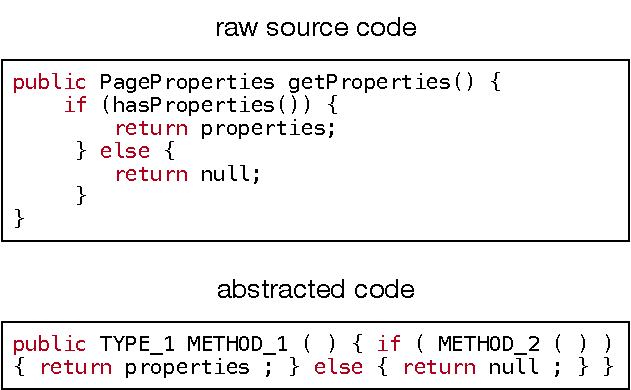
\includegraphics[width=0.37\linewidth]{eg_abs}
	\caption{Example of abstraction.}
	\label{fig:abstraction}
	\vspace{-0.1cm}
\end{figure}

The model was evaluated using quantitative metrics and qualitative analysis:
\begin{enumerate}
	\item Number of perfect predictions: prediction is considered ``perfect'' if the
	      generated revised code is identical to the expected code written.
	\item BLEU-4 score: measures the overlap between the model's output and the reference
	      revised code at the n-gram level (up to 4-grams).
	\item Levenshtein Distance: the minimum number of token edits (insertions, deletions,
	      or substitutions) needed to transform the model's output into the reference
	      code.
\end{enumerate}

%The results reveal that the reviewers comment helped a lot the model's accuracy,
%offering a $4\times$ improvement for a beam size equal to 1 (considering the
%only the token with the highest probability) and a $2\times$ for a beam size of
%10 (considering the top-10 tokens). The 2-encoder model (the one considering
%both the submitted code and the reviewers comment) had a 30\% accuracy on the
%perfect predictions, with an average of 0.91 BLEU-4 score and 0.09 Levenshtein
%distance over all the predictions.

The results reveal that the reviewers comment helped a lot the model's
accuracy, offering a $4\times$ improvement when considering the only prediction
with highest probability and a $2\times$ improvement when considering the
top-10 predictions, compared to the model receiving no reviewers' feedback in
input.

% This model obtained a 30\% accuracy on the perfect predictions, with an average
% of 0.91 BLEU-4 score and 0.09 Levenshtein distance over all the predictions.

Patanamon \etal \cite{patanamon:icse2022} and Tufano \etal
\cite{tufano:icse2022} showed that using more advanced techniques such as
Byte-Pair Encoding and transformer models can substantially enhances the
automation of this task.

%Neural Machine Translation significantly enhances performance, addressing
%challenges with out-of-vocabulary terms and large vocabulary sizes.
%Additionally,  showed that using the
%Text-To-Text Transfer Transformer (T5) model can also effectively support the
%code review process, particularly for tasks involving code revision.

\subsubsection{Code Quality Check}

Under the task of ``code quality checks'' we can factor a variety of methods
aimed at partially automating the assessment of code quality during reviews.
Researchers have developed different approaches to evaluate the quality of code
changes, although these approaches vary widely in terms of complexity and
scope.

One common approach in this area is \textit{Predicting Code Defectiveness},
which focuses on identifying potential bugs within code changes. For example,
Sharma \etal explored methods to predict whether a given code change may
introduce defects \cite{sharma:spe2019}. Similarly, Soltanifar \textit{et al.}
applied different classical machine learning techniques, such as Logistic
Regression, Naive Bayes, and Bayesian Networks, to this task, concluding that
Bayesian Networks achieved the best performance with 76\% accuracy in
predicting defectiveness \cite{soltanifar:esem2016}.

Another area of focus is \textit{Identifying Clone Refactoring Opportunities}.
Chen \etal proposed Pattern-based Clone Refactoring Inspection (PRI), a
technique that leverages refactoring pattern templates to identify clone
refactoring opportunities with high accuracy. PRI achieved 94.1\% accuracy in
identifying clone refactorings and 98.4\% in detecting inconsistencies within
these refactorings \cite{chen:compsac2017}. Additionally, Jiantao \textit{et
	al.} developed a tool aimed at checking consistency in design patterns, which
further supports refactoring efforts \cite{he:sere2013}.

In \textit{Predicting Problematic Code Lines}, researchers focus on identifying
specific lines in code that may be error-prone, to improve the review process
by flagging these lines early. Hong \etal developed a tool using machine
learning techniques to predict problematic code lines, achieving a Top-10
Accuracy of 81\% and 93\% for different scenarios. This approach allows
reviewers to concentrate on potentially problematic lines first, making the
review process more efficient.

Some researchers focused on \textit{Reviewing via Static Analysis}, applying
static analysis tools to detect issues such as code formatting violations or
potential errors. For instance, Balachandran \etal applied static analysis to
generate review comments, and Markovtsev \etal developed methods to suggest
fixes for code formatting violations, further automating quality checks during
code reviews \cite{balachandran:icse2013,markovtsev:msr2019}.

Finally, a recent trend involves \textit{Generating Review Comments} using deep
learning models to provide natural language feedback on code patches,
simulating human reviewer comments. These models are trained on large datasets
of prior code reviews and changes, allowing them to generate relevant comments
for new changes. We discuss in details the main papers addressing this task in
the following.

\paragraph{Using Pre-Trained Models to Boost Code Review Automation}

In 2022, Tufano \etal~\cite{tufano:icse2022} overcome the limitations discussed
in Section \ref{sub:revised} about their previous work \cite{tufano:icse2021}
by leveraging a pre-trained \textit{Text-to-Text Transfer Transformer} (T5)
model~\cite{raffel:jmlr2019}. Unlike previous approaches, the T5 model works
directly with raw source code without the need for code abstraction, thus
supporting more complex review. This is achieved by training T5 on a
substantially larger dataset that include a variety of realistic code review
transformations, including those requiring the introduction of new identifiers
and literals.

Empirical results show that the T5 model significantly outperforms the authors'
earlier deep learning models, particularly in scenarios involving complex code
changes. The study highlights the role of pre-training in enhancing
performance, especially in tasks involving natural language, such as generating
or interpreting comments.

However, while this approach marks a substantial improvement, the authors
acknowledge that current performance levels do not yet make T5 suitable for
deployment in real-world code review processes. They suggest that future works
should focus on increasing the accuracy of predictions, possibly by integrating
confidence-based filtering to prioritize high-quality recommendations and
combining various representations of code.

The T5 model was pre-trained on a refined corpus made from a cleaned and
filtered version of the official Stack Overflow Dump \cite{so_dump} and
CodeSearchNet \cite{Java:CodeSearchNet}. It was comprised 1,485,326 instances
of technical English, only related to Java code, and was used for pre-training
via masked token prediction.

For fine-tuning, the model used a dataset of 167,799 triplets from Java
open-source projects on GitHub and Gerrit. The dataset is of the same form as
the one from their previous work \cite{tufano:icse2021} discussed in
Section~\ref{sub:revised}, but without the abstraction process.

The model evaluation was conducted on a dataset of 16,780 instances. The
primary metric was "perfect predictions," meaning cases where the model’s
output exactly matched the expected output of the specified tasks. They also
used the BLEU (Bilingual Evaluation Understudy) score \cite{papineni2002bleu}
to evaluate the similarity between the generated review and the expected one,
however it didn't turn out to be very useful, given the low number of perfect
matches.

The authors also conducted a more in-depth analysis by examining 100 instances
where the model predictions did not achieve a perfect match with the target
output in the triplet. For the code-to-comment task, 36 instances were found to
be semantically equivalent, and 10 were alternative solutions. This analysis
indicates that perfect matches represent only a lower bound of the model's
potential performance, as many predictions classified as "wrong" were in fact
correct but formulated differently.

\paragraph{CommentFinder: A Simpler, Faster, More Accurate Code Review Comments Recommendation}

Hong \emph{et al.} \cite{hong:esecfse2022} introduced CommentFinder, a
retrieval-based approach to recommending code review comments for software
development. The approach addresses limitations in prior deep learning
(DL)-based methods \cite{tufano:icse2022}, which, while promising, are
computationally expensive and resource-intensive. CommentFinder uses
information retrieval techniques to recommend comments by finding similarities
between code changes and their associated review comments in a pre-existing
dataset, significantly reducing computational demands and time.

CommentFinder operates in three primary steps: vectorizing code changes using a
Bag-of-Words model, retrieving the most similar methods based on cosine
distance, and refining the results with Gestalt Pattern Matching (GPM) to
recommend the most relevant comments. This process eliminates the need for a
training phase, distinguishing it from the DL-based approaches that require
substantial computational resources for training.

The tool has been trained on the same dataset as the one from Tufano \textit{et
	al.} \cite{tufano:icse2022} and uses the same evaluation methods. CommentFinder
outperformed the DL approach, achieving 32\%-51\% higher perfect predictions
and 3\%-28\% higher BLEU scores. Additionally, CommentFinder was 49 times
faster in computational time, taking only 4 minutes compared to 194 minutes for
the DL model.

\paragraph{AUGER: Automatically Generating Review Comments with Pre-training Models}

Li \emph{et al.} \cite{li.l:esecfse2022} introduced AUGER, a review generator
similar to what Tufano \etal has done \cite{tufano:icse2022}, since it uses a
T5 model, but on a coarser level, as it aims to focus on review lines instead
of functions.

The dataset used to train AUGER comprises 10,882 code changes extracted from 11
influential Java projects on GitHub, amounting to 79,344 manually curated
review comments. The authors employ extensive preprocessing, including semantic
augmentation and heuristic filtering, to ensure the dataset's quality. The
training process incorporates fine-tuning the T5 model to understand
correlations between code changes and their respective review comments. This
approach allows for the generation of comments tailored to specific lines of
code rather than broader functional segments.

To evaluate AUGER, the authors conduct experiments using metrics such as
ROUGE-L and perfect prediction rates. AUGER outperforms baseline models,
achieving a 37.38\% improvement in ROUGE-L over traditional methods, such as
LSTM and CodeBERT. Additionally, case studies demonstrate that 29\% of its
generated comments are rated as useful, aligning closely with human reviewer
performance. The model's ability to generate comments in under 20 seconds
highlights its practical efficiency compared to manual review.

\paragraph{Automating Code Review Activities by Large-Scale Pre-training}

Li \emph{et al.} \cite{li.l:esecfse2022} introduced CodeReviewer, a pre-trained
encoder-decoder model specifically designed for automating key aspects of the
code review process. This includes tasks such as code change quality
estimation, review comment generation, and code refinement. The model builds on
a transformer-based architecture, leveraging advancements in large-scale
pre-training to tackle the complexity of code review tasks effectively.

CodeReviewer was trained on a novel dataset constructed from GitHub pull
requests, covering code changes and their corresponding review comments across
nine popular programming languages (C, C++, C\#, Go, Java, JavaScript, PHP,
Python and Ruby). In total, the dataset consists of approximately 7.9 million
pull requests from 1,161 high-quality repositories. This multilingual dataset
is not only extensive but also meticulously curated to ensure high-quality data
for both pre-training and downstream evaluation. To have a more effective
pre-training process, it was was divided into four steps: diff tag prediction,
denoising code diff, denoising review comments, and review comment generation.
This was made enhance the model's capacity to understand and interact with the
unique structures of code diffs and reviews. The dataset formation involved
extensive preprocessing to align code changes with corresponding review
comments. Code changes were represented using the "diff hunk" format, which
highlights added, deleted, and unchanged lines, making the dataset particularly
suitable for the code review scenario. Comments authored by the contributors
themselves were excluded to focus solely on reviewer input. To enhance the
relevance of the code refinement dataset, triplets of (original code, review
comment, revised code) were extracted from commits, ensuring that the model
could learn from meaningful revisions influenced by reviewer feedback.

The evaluation benchmarks demonstrated that CodeReviewer consistently
outperformed state-of-the-art models in all three targeted tasks. For code
change quality estimation, the model exhibited superior precision and F1
scores, reflecting its ability to effectively prioritize potentially
problematic code segments. In review comment generation, CodeReviewer produced
comments with higher informativeness and relevance scores compared to its
competitors, as validated through both automated metrics and human evaluation.
Similarly, in the code refinement task, it achieved a notable increase in BLEU
scores and perfect prediction rates, showcasing its ability to assist
developers in implementing reviewer feedback accurately.

\subsubsection{Assessing Review Quality}

While previous research has primarily focused on assisting the review process
by providing reviewers with additional information or reducing their workload,
studies in this area aim to evaluate the quality of the reviews themselves.
This line of research seeks to give feedback to reviewers, allowing them to
improve the effectiveness of their comments and suggestions where necessary.

% NOTE: this might be useful for us to determine which reviews are useful,
% especially what Pangsakulyanont did (?) and maybe also Rahman
One approach in this area involves \textit{Classifying the Usefulness of Review
	Comments}, which determines whether a review comment is helpful to the
contributor. Hasan \etal \cite{hasan:emse2021} investigated this classification
in an industrial setting, while Pangsakulyanont \textit{et
	al.}\cite{pangsakulyanont:iwesep2014} explored similar techniques within
open-source software environments. Additionally, Rahman \etal
\cite{rahman:msr2017} developed a prediction model called RevHelper to assess
comment usefulness, testing it on a dataset of 1,482 reviews and achieving an
accuracy of 66\% in predicting whether a review comment would be useful.

Another related task is \textit{Identifying Review Comments Needing Further
	Explanations}, which focuses on identifying comments that may be unclear and
thus require more detail to be fully understood by the contributor. Rahman
\etal \cite{rahman:esem2022} addressed this challenge by analyzing review
comments that lacked sufficient context, allowing contributors to take specific
action for clarification.

\subsubsection{Code Review Sentiment Analysis}

During the code review process, a developer (reviewer) may provide critiques
directed at a peer (contributor). The way these critiques are expressed in the
reviewer’s comments can significantly impact the success of the entire review
process. To support this, researchers have applied sentiment analysis
techniques to automatically classify the tone of reviewers' comments
\cite{ahmed:ase2017}: Flagging comments with negative sentiments offers
valuable feedback to reviewers, allowing them to reconsider potentially
problematic remarks. Similarly, Egelman \etal \cite{egelman:icse2020} focus on
identifying a specific subset of negative comments, \ie those that suggest a
reviewer’s intent to block a change request due to interpersonal conflicts
rather than issues with the quality of the submitted code.

\subsubsection{Retrieval of Similar Code Reviews/Code Changes}
Retrieval techniques have been applied to create recommender systems that
support code review in various ways. For example, when a code fragment is up
for review, some methods \cite{guo2020review,gupta:sigkdd2018,siow:saner2020}
pull up past reviews of similar code fragments and suggest reusable comments to
the reviewer, as these comments were previously used to recommend improvements
for similar code. Rahman \etal \cite{rahman:esem2022} proposed a similar
approach, but with a focus on helping the contributor by providing examples of
reviews similar to the feedback they’re receiving, which can help them better
understand the reviewer’s suggestions. On the other hand, Ueda \etal
\cite{ueda:iwsc2019} concentrated on identifying common improvement patterns in
code reviews—frequent changes that reviewers recommend. These patterns could
potentially be applied to enhance the code quality even before the review
begins.

\subsubsection{Time Management}
Research shows that both open-source and industrial projects can involve
hundreds of reviews each month. In such a high-volume environment, managing
time efficiently is crucial, and researchers have proposed solutions to help
allocate reviewers’ time more effectively. Unlike previous techniques focused
on automating specific review tasks, these approaches aim to enhance the
information available to reviewers and managers, potentially leading to better
decision-making in the review process.

Some of these solutions can be combined into a pipeline to streamline code
review. For instance, methods for predicting the time needed to complete a pull
request \cite{maddila:esefse2019,shan:esecfse2022} make it possible to identify
overdue requests \cite{shan:esecfse2022}, meaning those taking longer than
anticipated. These flagged pull requests can then be analyzed using techniques
that identify the "blocking actor(s)" \cite{shan:esecfse2022}—individuals
responsible for the delay—enabling teams to either prompt action or, if
feasible, reassign the task.

\subsection{Benchmarks to Assess DL-based Solutions for Code-related Tasks}

Table~\ref{tab:benchs} provides an overview of key benchmarks designed to
evaluate DL-based solutions for various code-related tasks, including code
generation, code editing, and multitask capabilities. The table categorizes
these benchmarks by task type, release year, dataset size, and supported
programming languages. These benchmarks serve as critical tools for assessing
the performance and practicality of DL models in software engineering contexts.
We will delve into the specifics of each benchmark to better understand their
design, scope, and significance.

\begin{table}[ht]
	\centering
	\begin{tabular}{llrrl}
		\toprule
		\textbf{Category}     &
		\textbf{Name}         &
		\textbf{Release}      &
		\textbf{\# instances} &
		\textbf{Languages}                                                                                              \\
		\midrule
		Code Generation       & HumanEval \cite{chen2021}                     & 2021 & 164       & Python               \\
		                      & MultiPL-E \cite{cassano2022}                  & 2023 & 164       & 18 languages         \\
		                      & CoderEval \cite{Zhang_2024}                   & 2024 & 230 + 230 & Python + Java        \\
		\arrayrulecolor{lightgray}\hline
		Code Editing          & SWE-bench \cite{jimenez2024swebench}          & 2024 & 2,294     & Python               \\
		                      & DebugBench \cite{tian2024debugbench}          & 2024 & 4,253     & C++, Java and Python \\
		                      & CodeEditorBench \cite{guo2024codeeditorbench} & 2024 & 7,961     & C++, Java and Python \\
		\arrayrulecolor{lightgray}\hline
		Multitask             & CoderUJB \cite{zeng2024coderujb}              & 2024 & 2,239     & Java                 \\
		\arrayrulecolor{black}\bottomrule
	\end{tabular}
	\caption{Benchmarks to Assess DL-based Solutions for Code-related Tasks}\label{tab:benchs}
\end{table}

\subsubsection{Code generation}

\paragraph{HumanEval \cite{chen2021}}
HumanEval is used to measure functional correctness for synthesizing programs from
docstrings. It consists of 164 original programming problems, assessing
language comprehension, algorithms, and simple mathematics, with some
comparable to simple software interview questions.

\paragraph{MultiPL-E \cite{cassano2022}}
MultiPL-E is a multi-programming language benchmark for evaluating the code
generation performance of large language model (LLMs) of code. It expands on
the previous benchmark by translating the problems into 18 different
programming languages.

\paragraph{CoderEval \cite{Zhang_2024}}
CoderEval is a code generation benchmark to evaluate the performance
of generative pre-trained models. Compared with the widely-used HumanEval
benchmark from OpenAI, CoderEval can be used to evaluate the performance of
models against pragmatic code generation beyond just generating standalone
functions. It is comprised 230 functions from 43 Python projects and 230 methods
from 10 Java projects. For each function/method, the authors extracted the original
docstring/comment, the signature, the code implementation, and the corresponding
test code (if exists) to form one function-level code generation task. CoderEval
can be viewed as a superset of HumanEval.

\subsubsection{Code editing}

\paragraph{SWE-bench \cite{jimenez2024swebench}}
SWE-Bench is a benchmark designed to evaluate the capabilities of language
models in addressing real-world software engineering problems sourced from
GitHub. It comprises 2,294 tasks derived from issues and pull requests in 12
popular Python repositories. These tasks require models to edit large and
complex codebases to resolve bugs or implement new features, often demanding
context comprehension across multiple files, execution environment interaction,
and sophisticated reasoning. Solutions are evaluated using repository-specific
tests, with success measured by the resolution of predefined "fail-to-pass"
tests. Despite its rigor, state-of-the-art models show limited performance,
highlighting SWE-Bench's value as a challenging benchmark for advancing language
models' practical software engineering capabilities.

\paragraph{DebugBench \cite{tian2024debugbench}}
DebugBench is a benchmark designed to evaluate the debugging capabilities of
large language models (LLMs) through 4,253 instances of buggy code. Covering
three programming languages: C++, Java, and Python. DebugBench categorizes bugs
into four major groups (Syntax, Reference, Logic, and Multiple errors) and 18
subtypes. The dataset is derived from code snippets on LeetCode and enhanced
with synthetic bugs implanted by GPT-4. Rigorous filtering and manual
inspections ensure the integrity and diversity of the dataset. Evaluations
using both closed-source and open-source LLMs reveal significant gaps in
debugging performance compared to humans, especially for logic and multiple
errors. DebugBench highlights the potential for runtime feedback and its
varying effects across bug types, providing a robust platform for advancing LLM
debugging capabilities.

\paragraph{CodeEditorBench \cite{guo2024codeeditorbench}}
CodeEditorBench is a benchmark designed to assess the code editing capabilities
of LLMs across four key tasks: debugging, translating,
polishing, and requirement switching. It incorporates a dataset of 7,961 tasks
derived from sources such as LeetCode and CodeNet, enriched with test cases
generated by LLMs and validated by an online judge system. Evaluations of 19
LLMs reveal significant performance disparities, with closed-source models like
GPT-4 excelling in debugging and translating, while challenges persist in
polishing and requirement adaptation tasks.

\subsubsection{Multitask}

\paragraph{CoderUJB \cite{zeng2024coderujb}}
CoderUJB is a comprehensive benchmark tailored to evaluate the programming
capabilities of LLMs in realistic Java-based development
scenarios. Built from 17 open-source Java projects, it comprises 2,239
programming tasks spanning five areas: functional code generation, code-based
test generation, issue-based test generation, defect detection, and automated
program repair. Each task is executable and evaluated within a complete project
context, reflecting real-world software engineering challenges. The benchmark
also assesses the impact of pre-training and instruction fine-tuning on LLM
performance, revealing gaps in handling non-functional code tasks like defect
detection.

\subsection{Summing up}

Our benchmark introduces two key innovations compared to the previously
discussed benchmarks. First, there are currently no benchmarks explicitly
designed to evaluate the generation of code review comments. Second, none of
the existing benchmarks, even those about code editing, exercise models in the
task of addressing a given code review comment expressed in natural language.
Our objective is to assess the quality of generated code by considering both
the submitted code and the accompanying reviewer's comments.

We expect the proposed benchmark to substantially increase the reliability of
empirical evaluations performed on deep learning-based code review automation
tools.
